\documentclass[12pt]{beamer}
\usepackage{pgf}
\usepackage[danish]{babel}
\usepackage[utf8]{inputenc}
\usepackage{beamerthemesplit}
\usepackage{graphics,epsfig, subfigure}
\usepackage{url}
\usepackage{srcltx}
\usepackage{hyperref}
\usepackage{fancybox}
\usepackage{listings}
\lstset{
  language=C,                % choose the language of the code
   basicstyle=\footnotesize,        % the size of the fonts that are used for the code
    keywordstyle=\color{blue},       % keyword style
     commentstyle=\color[rgb]{0.13,0.54,0.13},
  numbers=left,                   % where to put the line-numbers
  stepnumber= 0.3,                   % the step between two line-numbers.        
  numbersep=1pt,                  % how far the line-numbers are from the code
  backgroundcolor=\color{white},  % choose the background color. You must add \usepackage{color}
  showspaces=false,               % show spaces adding particular underscores
  showstringspaces=false,         % underline spaces within strings
  showtabs=false,                 % show tabs within strings adding particular underscores
  tabsize=2,                      % sets default tabsize to 2 spaces
  captionpos=b,                   % sets the caption-position to bottom
  breaklines=true,                % sets automatic line breaking
  breakatwhitespace=true,         % sets if automatic breaks should only happen at whitespace
 % title=\lstname,                 % show the filename of files included with \lstinputlisting;
}
\definecolor{kugreen}{RGB}{50,93,61}
\definecolor{kugreenlys}{RGB}{132,158,139}
\definecolor{kugreenlyslys}{RGB}{173,190,177}
\definecolor{kugreenlyslyslys}{RGB}{214,223,216}
\setbeamercovered{transparent}
\mode<presentation>
\usetheme[numbers,totalnumber,compress,sidebarshades]{PaloAlto}
\setbeamertemplate{section in toc}[sections numbered]

\setbeamertemplate{footline}[frame number]

  \usecolortheme[named=kugreen]{structure}
  \useinnertheme{circles}
  \usefonttheme[onlymath]{serif}
  \setbeamercovered{transparent}
  \setbeamertemplate{blocks}[rounded][shadow=true]

\logo{
\includegraphics[width=0.8cm]{fga_logo.png}}
%\useoutertheme{infolines} 
\title{Gestão de Portfólios e Projetos de Software}
\subtitle{Fases ou Grupos de Processo: Planejamento II}
\author{Dra. Carla Rocha, Msc. Hilmer R. Neri}


\institute{Engenharia de Software \\ Universidade de Brasília}
\date{2015.2}


\begin{document}
\frame{\titlepage \vspace{-0.5cm}	
}
\frame
{
\frametitle{Agenda}
\tableofcontents%[pausesection]
}
\section{Grupo de Processo Planejamento}

\begin{frame}
 \frametitle{GRUPO DE PROCESSOS (“FASE”) – PLANEJAMENTO}
  \begin{figure}
   \centering
   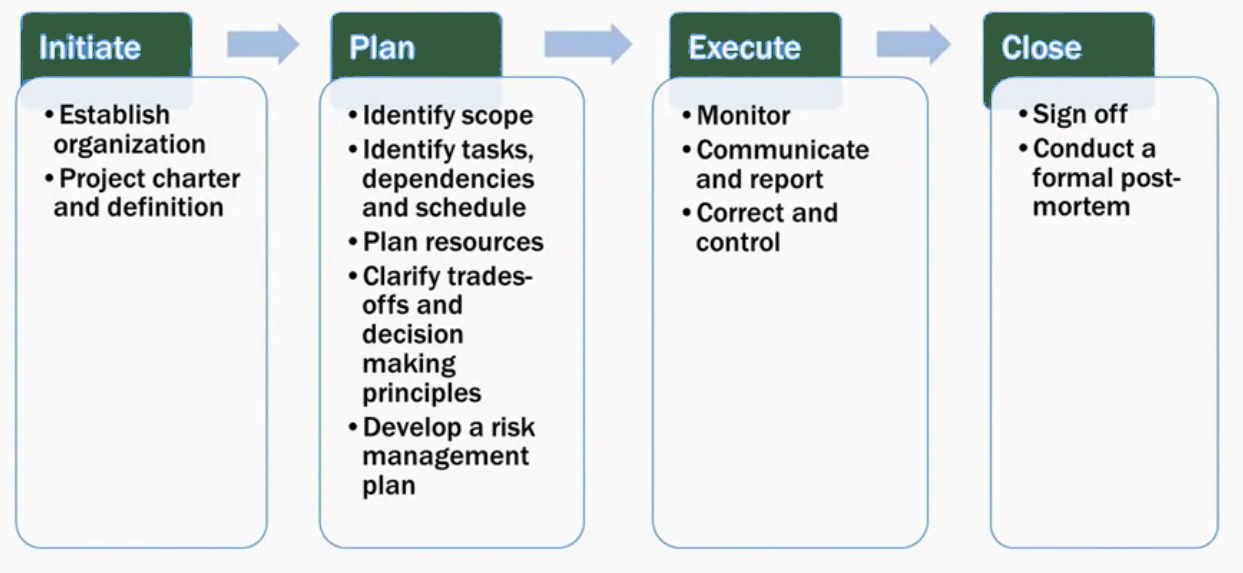
\includegraphics[width = 0.9\textwidth]{figs/fig0.png}
  \end{figure}
\end{frame}

\begin{frame}
 \frametitle{Grupo de Processos de planejamento}
 \begin{block}{Definição PMBok}
  O grupo de processos de planejamento consiste dos \textbf{processos} realizados para estabelecer o \textbf{escopo}
total do esforço, definir e refinar os \textbf{objetivos} e desenvolver o  \textbf{curso de ação necessário} para alcançar esses
objetivos.
 \end{block}
\end{frame}

\begin{frame}
 \frametitle{Grupo de Processos de planejamento}
 \begin{block}{Definição PMBok}
 Os processos de planejamento desenvolvem o \textbf{plano de gerenciamento} e os \textbf{documentos} do projeto
que serão \textbf{usados para executá-lo}
 \end{block}
\end{frame}

\begin{frame}
 \frametitle{Grupo de Processos de planejamento}
 \begin{block}{Definição PMBok}
O \textbf{benefício principal} deste grupo de
processos é \textbf{delinear a estratégia e a tática}, e também o \textbf{curso de ação} ou o caminho para a conclusão do
projeto ou da fase com sucesso.
\end{block}
\end{frame}

\begin{frame}
 \frametitle{GRUPO DE PROCESSOS (“FASE”) – PLANEJAMENTO}
  \begin{figure}
   \centering
   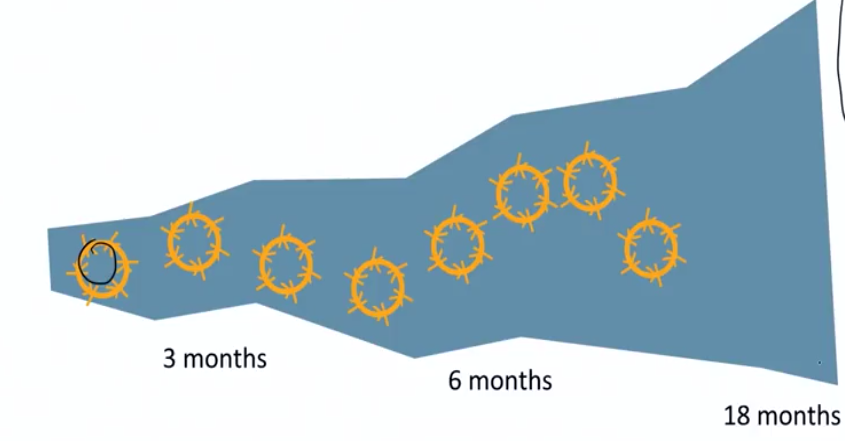
\includegraphics[width = 0.9\textwidth]{figs/fig14.png}
   \caption{Fluxograma}
  \end{figure}
\end{frame}

\begin{frame}
 \frametitle{GRUPO DE PROCESSOS (“FASE”) – PLANEJAMENTO}
  \begin{figure}
   \centering
   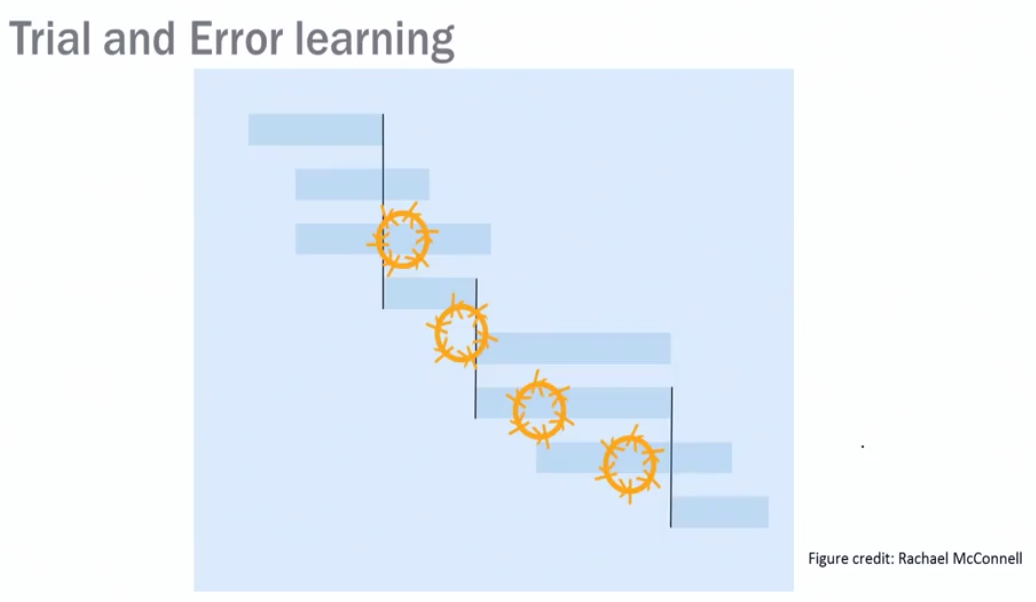
\includegraphics[height = 0.9\textheight]{figs/fig15.png}
  \end{figure}
\end{frame}

\begin{frame}
 \frametitle{GRUPO DE PROCESSOS (“FASE”) – PLANEJAMENTO}
  \begin{figure}
   \centering
   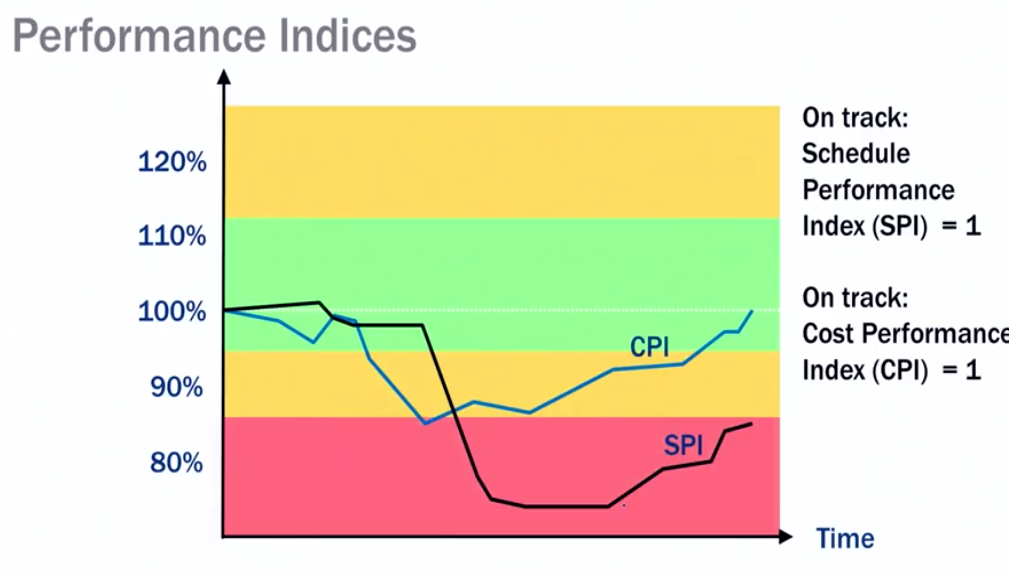
\includegraphics[height = 0.9\textheight]{figs/fig16.png}
   \caption{Fluxograma}
  \end{figure}
\end{frame}
\begin{frame}
 \frametitle{GRUPO DE PROCESSOS (“FASE”) – PLANEJAMENTO}
  \begin{figure}
   \centering
   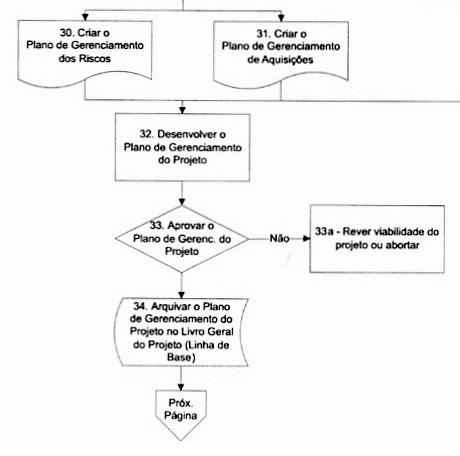
\includegraphics[height = 0.9\textheight]{figs/fig17.png}
   \caption{Fluxograma}
  \end{figure}
\end{frame}

\section{Definir e Agrupar as Atividades}

\begin{frame}
 \frametitle{GRUPO DE PROCESSOS (“FASE”) – PLANEJAMENTO}
   14 – Definir e Agrupar as Atividades que Serão Executadas pelo Projeto (WBS -  Work Breakdown Structure)
  \begin{block}{Definição EAP}
 É a decomposição hierárquica do escopo total do trabalho a ser executado pela equipe do projeto a fim
 de alcançar os objetivos do projeto e criar entregas exigidas
  \end{block}
\end{frame}

\begin{frame}
 \frametitle{GRUPO DE PROCESSOS (“FASE”) – PLANEJAMENTO}
   14 – Definir e Agrupar as Atividades que Serão Executadas pelo Projeto (WBS -  Work Breakdown Structure)
  \begin{itemize}
   \item Visualmente quebra o escopo do projeto no formato de uma árvore
   \begin{enumerate}
    \item O componente mais geral para o mais específico
    \item Fases do ciclo de vida do projeto
    \item Pacotes de Trabalho
    \item Atividades/Tarefas
   \end{enumerate}
  \end{itemize}
\end{frame}

\begin{frame}
 \frametitle{GRUPO DE PROCESSOS (“FASE”) – PLANEJAMENTO}
   14 – Definir e Agrupar as Atividades que Serão Executadas pelo Projeto (WBS -  Work Breakdown Structure)
  \begin{block}{Obejtivo EAP}
 Identificar elementos terminais (produtos/serviços), clarificando e definindo o escopo total do projeto. \textbf{Fornece uma linha de base
 para o controle de mudanças no projeto}
  \end{block}
\end{frame}

\begin{frame}
 \frametitle{GRUPO DE PROCESSOS (“FASE”) – PLANEJAMENTO}
   14 – Definir e Agrupar as Atividades que Serão Executadas pelo Projeto (WBS)
  \begin{itemize}
   \item Definição de uma Boa EAP:
   \begin{itemize}
    \item Estrutura não baseada em tempo
    \item Elementos orientados a entregas
    \item Não orientada a processos
    \item Define a relação lógica entre componentes
    \item Nome elementos são "substantivos" (nunca verbos)
    \item Atividades do projetos não estão na EAP
    \item Deve incluir apenas entrega (deliverables) necessários e suficientes 
   \end{itemize}
  \end{itemize}
\end{frame}

\begin{frame}
 \frametitle{GRUPO DE PROCESSOS (“FASE”) – PLANEJAMENTO}
   14 – Definir e Agrupar as Atividades que Serão Executadas pelo Projeto (WBS)
  \begin{itemize}
   \item Características da EAP:
   \begin{itemize}
    \item Permite que se veja a contribuição dos pacotes de trabalho
    \item Permite o direcionamento das equipes, dos recursos e das responsabilidades
    \item Determina quais materiais serão necessários para a execução de cada equipe
    \item Determina o custo final do projeto a partir do custo de cada pacote ou entrega
   \end{itemize}
  \end{itemize}
\end{frame}

\begin{frame}
 \frametitle{GRUPO DE PROCESSOS (“FASE”) – PLANEJAMENTO}
   14 – Definir e Agrupar as Atividades que Serão Executadas pelo Projeto (WBS)
  \begin{itemize}
   \item Principais vantagens da EAP:
   \begin{itemize}
    \item Conjuntos de entregas agrupadas de forma simples
    \item Fácil atribuição de responsabilidades
    \item Fácil desmembramento do projeto em pacotes de trabalho
   \end{itemize}
  \end{itemize}
\end{frame}

\begin{frame}
 \frametitle{GRUPO DE PROCESSOS (“FASE”) – PLANEJAMENTO}
   14 – Definir e Agrupar as Atividades que Serão Executadas pelo Projeto (WBS)
  \begin{itemize}
   \item Principais desvantagens da EAP:
   \begin{itemize}
    \item Não diferencia, visualmente, o prazo e a duração de cada pacote, bem como a importância de cada um
    \item Não mostra as interdenpendências entre as entregas e os pacotes
   \end{itemize}
  \end{itemize}
\end{frame}

\begin{frame}
 \frametitle{GRUPO DE PROCESSOS (“FASE”) – PLANEJAMENTO}
   14 – Definir e Agrupar as Atividades que Serão Executadas pelo Projeto (WBS)
  \begin{itemize}
   \item A EAP pode ser detalhada na medida da necessidade do projeto. Os níveis mais comuns são apresentados a seguir
  \end{itemize}
  \begin{figure}
   \centering
   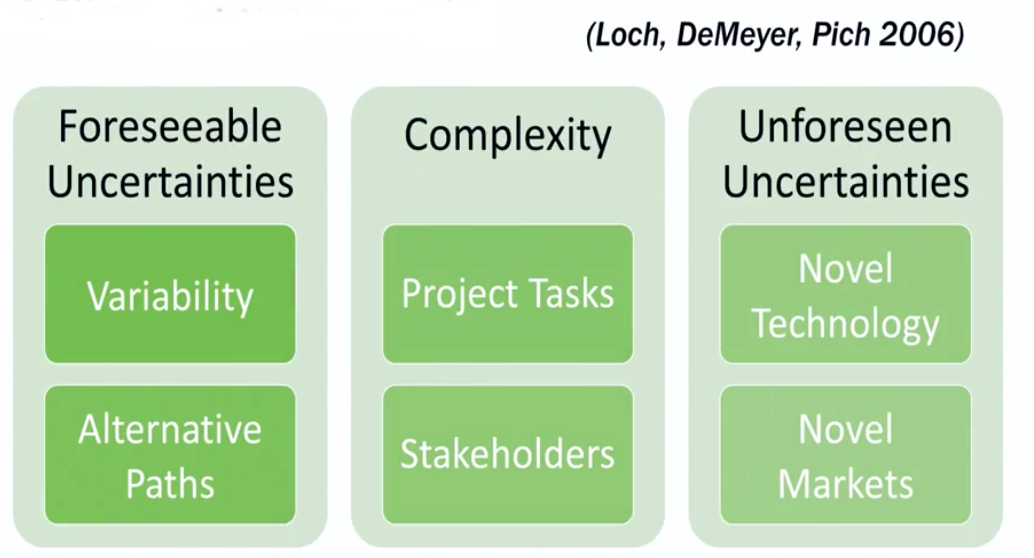
\includegraphics[width = 0.6\textwidth]{figs/fig1.png}
  \end{figure}
\end{frame}

\begin{frame}
 \frametitle{GRUPO DE PROCESSOS (“FASE”) – PLANEJAMENTO}
   14 – Definir e Agrupar as Atividades que Serão Executadas pelo Projeto (WBS)
  \begin{itemize}
   \item A EAP pode ser detalhada na medida da necessidade do projeto. 
  \end{itemize}
  Exemplos de projetos em semestres anteriores
\end{frame}

\begin{frame}
 \frametitle{GRUPO DE PROCESSOS (“FASE”) – PLANEJAMENTO}
   14 - Definir e Agrupar as Atividades que Serão Executadas pelo Projeto (WBS)
  \begin{itemize}
   \item Existem varias técnicas de estruturação das atividades para compor a EAP:
   \begin{itemize}
    \item Top-Bottom
    \item Bottom-Up
    \item Diagrama de causa e efeito (fish-bone)
    \item brainstorming
   \end{itemize}
  \end{itemize}
\end{frame}

\begin{frame}
 \frametitle{GRUPO DE PROCESSOS (“FASE”) – PLANEJAMENTO}
   14 - Definir e Agrupar as Atividades que Serão Executadas pelo Projeto (WBS)
  \begin{itemize}
   \item Existem duas técnicas de estruturação das atividades para compor a EAP:
   \begin{itemize}
    \item Top-to-Bottom ou Decomposição
    \begin{enumerate}
     \item Identificam-se as grandes fases do projeto
     \item Para cada entrega, detalha-se o pacote de trabalho necessário para sua conclusão
     \item Se necessário, para cada pacote de trabalho, detalha-se o nível de esforço localizado para conclusão do respectivo pacote
     \item Agregam-se os conjuntos de modo a produzir a EAP
    \end{enumerate}
   \end{itemize}
  \end{itemize}
\end{frame}

\begin{frame}
 \frametitle{GRUPO DE PROCESSOS (“FASE”) – PLANEJAMENTO}
   14 – Definir e Agrupar as Atividades que Serão Executadas pelo Projeto (WBS)
  \begin{itemize}
   \item Existem duas técnicas de estruturação das atividades para compor a EAP:
   \begin{itemize}
    \item Bottom-UP
    \begin{enumerate}
     \item obtém-se o conjunto de entregas através de brainstorming, ou através da experiência dos envolvidos
     \item criam-se os pacotes de trabalho para atingir as entregas
     \item agrupam-se as entregas em fases
     \item Agrupam-se as fases em um projeto
    \end{enumerate}
   \end{itemize}
  \end{itemize}
\end{frame}




\begin{frame}
 \frametitle{GRUPO DE PROCESSOS (“FASE”) – PLANEJAMENTO}
 14 – Definir e Agrupar as Atividades que Serão Executadas pelo Projeto (WBS)
  \begin{figure}
   \centering
   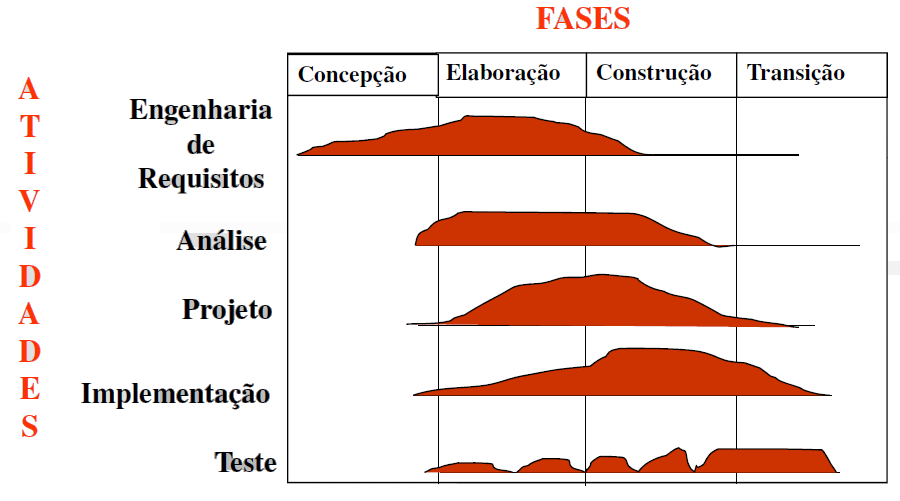
\includegraphics[width = 0.9\textwidth]{figs/fig19.png}
  \end{figure}
\end{frame}

\section{Criar a lista de atividades}
\begin{frame}
 \frametitle{GRUPO DE PROCESSOS (“FASE”) – PLANEJAMENTO}
18 – Criar a lista de atividades para os elementos do WBS
  \begin{block}{}
 Atividades são as etapas necessárias para se completar um projeto.  São executadas em uma sequência caracterizada pela natureza. Podem ocorrer sequencialmente ou simultaneamente
  \end{block}
  \begin{itemize}
   \item Os principais tipos de atividades são:
   \begin{itemize}
    \item Atividades executivas ou tarefas (tasks)
    \item Marcos ou entregas (Milestones)
    \item Atividades-resumo ou pacotes de trabalho (Summary tasks)
   \end{itemize}
  \end{itemize}
\end{frame}

\begin{frame}
 \frametitle{GRUPO DE PROCESSOS (“FASE”) – PLANEJAMENTO}
18 – Criar a lista de atividades para os elementos do WBS
  \begin{itemize}
   \item Atividades Executivas ou tarefas (tasks)
   \begin{itemize}
    \item São atividades relacionadas diretamente com a ação dentro do projeto
   \end{itemize}
   \item Marcos ou Entregas (milestones)
   \begin{itemize}
    \item Representam um evento, ou condição, que marca a execução de um grupo de atividades relacionadas entre si, ou término de uma fase do projeto
    \item Serve também para identificar as entregas dos pacotes de trabalho e não possui duração
   \end{itemize}
  \end{itemize}
\end{frame}

\begin{frame}
 \frametitle{GRUPO DE PROCESSOS (“FASE”) – PLANEJAMENTO}
18 – Criar a lista de atividades para os elementos do WBS
  \begin{itemize}
   \item Atividades-Resumo ou Pacote de Trabalho (summary tasks)
   \begin{itemize}
    \item São atividades que englobam outras atividades, chamadas de subatividades
    \item Representam conjunto de atividades, totalizando duração, datas e custos das atividades a elas pertencentes
    \item  Podem ser chamadas de pacotes de trabalho
   \end{itemize}
  \end{itemize}
\end{frame}

\begin{frame}
 \frametitle{GRUPO DE PROCESSOS (“FASE”) – PLANEJAMENTO}
18 – Criar a lista de atividades para os elementos do WBS
  \begin{figure}
   \centering
   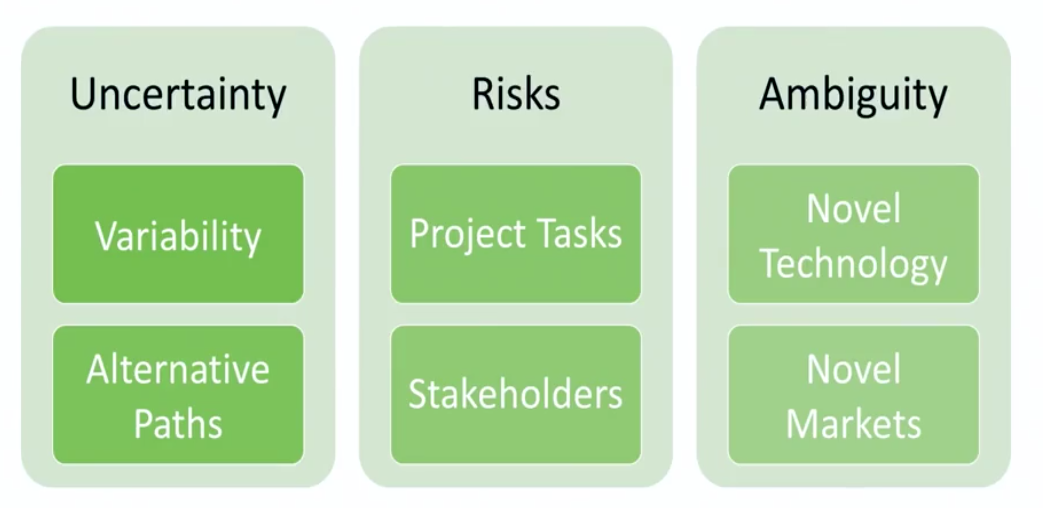
\includegraphics[width = 0.9\textwidth]{figs/fig2.png}
  \end{figure}
\end{frame}


\section{Determinar a duração das Atividades}
\begin{frame}
 \frametitle{GRUPO DE PROCESSOS (“FASE”) – PLANEJAMENTO}
19 – Determinar a duração das Atividades do Projeto
  \begin{block}{}
 A duração de uma atividade é o tempo necessário para que a atividade possa ser realizada. Pode ocorrer em semanas, dias, horas e minutos, dependendo de cada projeto
  \end{block}
  \begin{itemize}
   \item Para se calcular a duração do projeto é necessário que se conheçam todos os recursos alocados na atividade e a produtividade de cada um deles
  \end{itemize}
\end{frame}

\begin{frame}
 \frametitle{GRUPO DE PROCESSOS (“FASE”) - PLANEJAMENTO}
19 – Determinar a duração das Atividades do Projeto
  \begin{itemize}
   \item Estimar a duração das atividades é complexo:
   \begin{itemize}
    \item Lei de Parkinson -\textit{"O trabalho se expande de modo a preencher o tempo disponível para a sua realização."}
   \item Sindrome do Estudante
   \item Super confiança
   \item Biases : âncora, e confirmação
   \end{itemize} 
   \end{itemize} 
\end{frame}


\begin{frame}
 \frametitle{GRUPO DE PROCESSOS (“FASE”) - PLANEJAMENTO}
19 – Determinar a duração das Atividades do Projeto
  \begin{itemize}
   \item Segundo Lewis, estima-se que em um projeto, o tempo perdido é de 40\%
   \item Esse conceito é denominado \textbf{Fator de Produtividade}
  \end{itemize}
  \begin{block}{}
   O uso do fator de produtividade no cálculo da duração torna a atividade de estimativa mais realista.
  \end{block}
\end{frame}

\begin{frame}
 \frametitle{GRUPO DE PROCESSOS (“FASE”) – PLANEJAMENTO}
19 – Determinar a duração das Atividades do Projeto - \\
Atividades com Duração Fixa X Orientada para Recursos
  \begin{itemize}
   \item Atividades com duração Fixa X Atividades Orientadas para recursos
  \begin{itemize}
   \item Se um \textbf{recurso não influencia} a duração de uma atividade, essa atividade é denominada de duração fixa
   \item Já a atividade de orientada a recurso é aquela onde o \textbf{recurso influencia} a duração da atividade
  \end{itemize}
  \end{itemize}
\end{frame}

\begin{frame}
 \frametitle{GRUPO DE PROCESSOS (“FASE”) – PLANEJAMENTO}
19 – Determinar a duração das Atividades do Projeto - \\
Atividades com Duração Fixa X Orientada para Recursos
  \begin{figure}
   \centering
   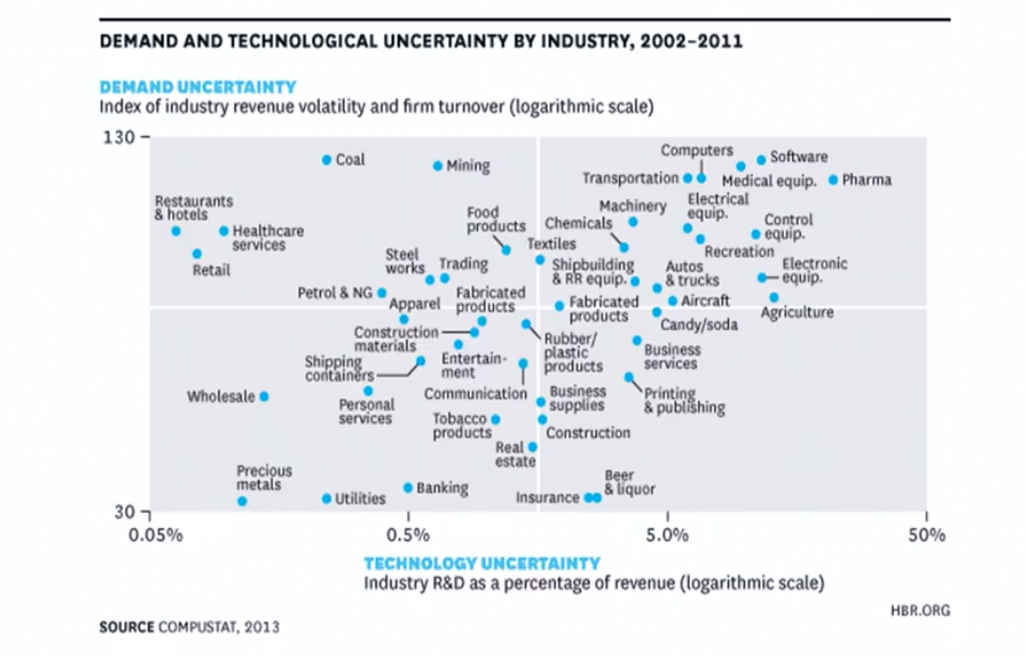
\includegraphics[width = 0.6\textwidth]{figs/fig3.png}
  \end{figure}
  \begin{itemize}
   \item O ato de aumentar a qtde. Recursos a fim de reduzir a duração é denominado \textbf{Compressão} ou \textbf{Crashing}
  \end{itemize}
\end{frame}

\begin{frame}
 \frametitle{GRUPO DE PROCESSOS (“FASE”) – PLANEJAMENTO}
19 – Determinar a duração das Atividades do Projeto - \\
Análise PERT
  \begin{itemize}
   \item Na análise PERT a duração de cada atividade é calculada através da estimativa da duração otimista, pessimista e mais provável, por meio de uma média ponderada
  \end{itemize}
  \begin{equation}
   Duracao = \frac{1 x Opt + 4 x Est + 1 x Pes }{6}
  \end{equation}
onde: Opt = duração otimista\\
               Est = duração mais provável\\
               Pes = duração pessimista
\end{frame}

\section{Definir Precedências}
\begin{frame}
 \frametitle{GRUPO DE PROCESSOS (“FASE”) – PLANEJAMENTO}
23 – Inter-relacionar as atividades e Definir Precedências
  \begin{itemize}
   \item O objetivo é associar as atividades, determinando suas dependências (sucessora e predecessora)
   \item Definições:
   \begin{itemize}
    \item Início do Projeto
    \item Término do Projeto
    \item Início da Atividade
    \item Término da Atividade
    \item Calendários
    \item Feriados e dias especiais
   \end{itemize}
  \end{itemize}
\end{frame}

\begin{frame}
 \frametitle{GRUPO DE PROCESSOS (“FASE”) – PLANEJAMENTO}
 23 – Inter-relacionar as atividades e Definir Precedências
 \begin{itemize}
  \item Matriz de dependência (design) estruturada (ex Startup)
 \end{itemize}
  \begin{figure}
   \centering
   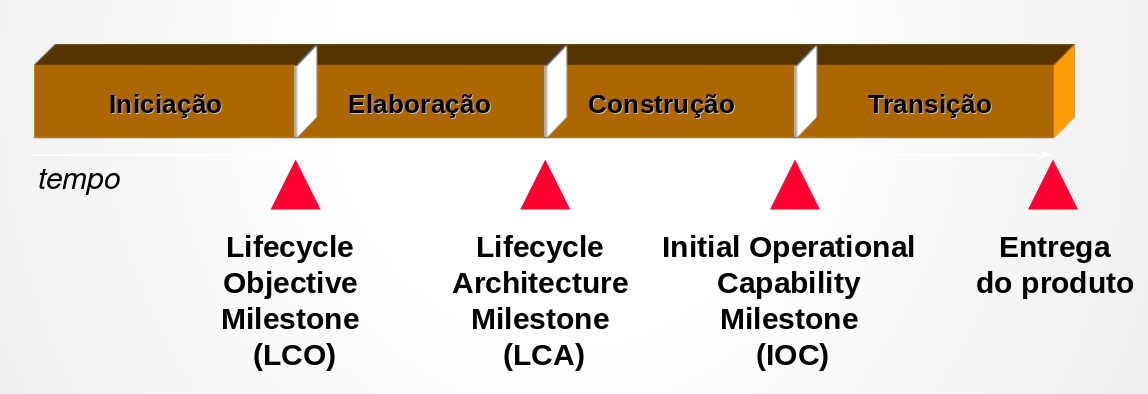
\includegraphics[width = 0.7\textwidth]{figs/fig20.png}
  \end{figure}
\end{frame}


\begin{frame}
 \frametitle{GRUPO DE PROCESSOS (“FASE”) – PLANEJAMENTO}
 23 – Inter-relacionar as atividades e Definir Precedências
 \begin{itemize}
  \item Matriz de dependência (ex Startup) - tabela
 \end{itemize}
  \begin{figure}
   \centering
   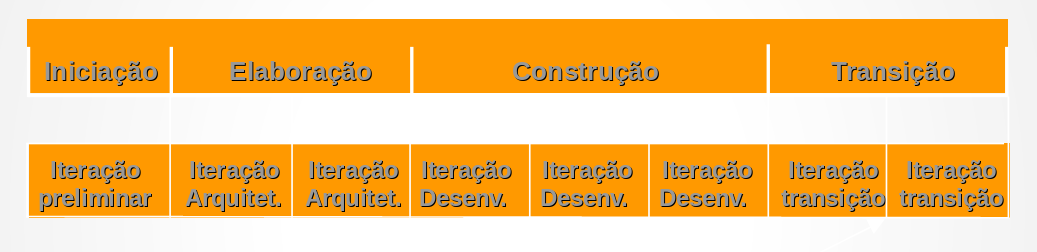
\includegraphics[width = 0.7\textwidth]{figs/fig21.png}
  \end{figure}
\end{frame}

\begin{frame}
 \frametitle{GRUPO DE PROCESSOS (“FASE”) – PLANEJAMENTO}
 23 – Inter-relacionar as atividades e Definir Precedências
 \begin{itemize}
  \item Matriz de dependência (ex Startup) - grafo
 \end{itemize}
  \begin{figure}
   \centering
   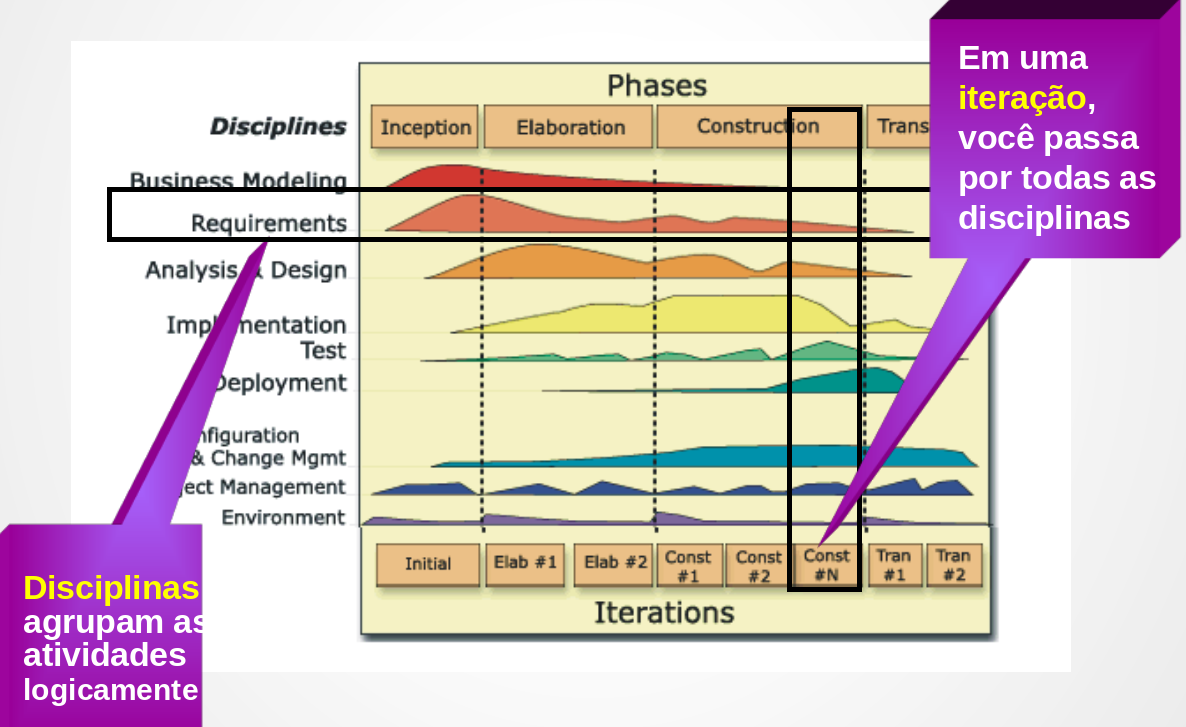
\includegraphics[width = 0.7\textwidth]{figs/fig22.png}
  \end{figure}
\end{frame}

\begin{frame}
 \frametitle{GRUPO DE PROCESSOS (“FASE”) – PLANEJAMENTO}
 23 – Inter-relacionar as atividades e Definir Precedências
 \begin{itemize}
  \item Matriz de dependência (ex Startup) - grafo
 \end{itemize}
  \begin{figure}
   \centering
   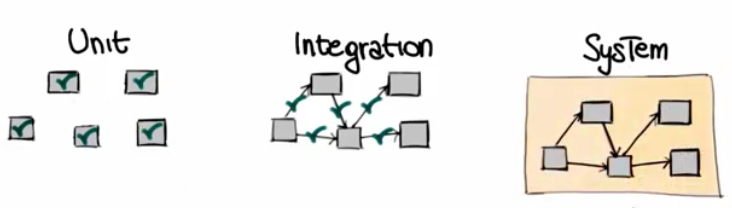
\includegraphics[width = 0.7\textwidth]{figs/fig23.png}
  \end{figure}
\end{frame}
\begin{frame}
 \frametitle{GRUPO DE PROCESSOS (“FASE”) – PLANEJAMENTO}
23 – Inter-relacionar as atividades e Definir Precedências-\\
Restrições de Datas nas Atividades
  \begin{itemize}
   \item As atividades podem ter diversos tipos de restrições quanto ao início ou término. São elas:
   \begin{itemize}
    \item Início o mais rápido possível (as soon as possible)
    \item Início o mais tarde possível (as late as possible)
    \item Início não antes de um determinado dia (start no earlier than)
    \item Início não depois de um determinado dia (start no later than)
    \item Início obrigatoriamente em uma data (must start on)
    \item Conlui, obrigatoriamente, em uma data (must finish on)
   \end{itemize}
  \end{itemize}
\end{frame}


\begin{frame}
 \frametitle{GRUPO DE PROCESSOS (“FASE”) – PLANEJAMENTO}
23 – Inter-relacionar as atividades e Definir Precedências-\\
Tipos de Inter-relacionamentos
  \begin{itemize}
   \item As atividades podem ser inter-relacionadas de várias formas. As principais são:
   \begin{itemize}
    \item Término para início – TI (finish to start – FS)
    \item Início para início – II (start to start – SS)
    \item  Término para término – TT (finish to finish – FF)
    \item Início para término – IT (start to finish – SF)
   \end{itemize}
  \end{itemize}
\end{frame}

\begin{frame}
 \frametitle{GRUPO DE PROCESSOS (“FASE”) – PLANEJAMENTO}
23 – Inter-relacionar as atividades e Definir Precedências-\\
Tipos de Inter-relacionamentos
  \begin{itemize}
   \item Término para início – TI (finish to start – FS)
   \begin{itemize}
    \item A atividade sucessora somente se \textbf{inicia} com o \textbf{término} da atividade predecessora
   \end{itemize}
  \end{itemize}
  \begin{figure}
   \centering
   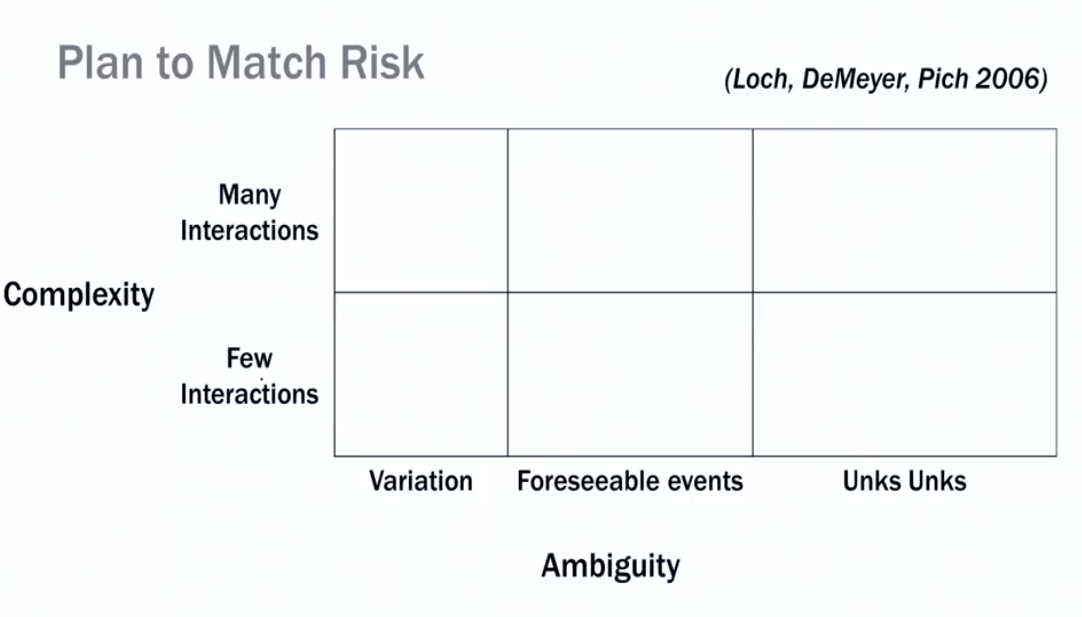
\includegraphics[width = 0.6\textwidth]{figs/fig4.png}
  \end{figure}
\end{frame}

\begin{frame}
 \frametitle{GRUPO DE PROCESSOS (“FASE”) – PLANEJAMENTO}
23 – Inter-relacionar as atividades e Definir Precedências-\\
Tipos de Inter-relacionamentos
  \begin{itemize}
   \item Início para início – II (start to start – SS)
   \begin{itemize}
    \item A atividade sucessora somente se inicia com o início da atividade predecessora
    \item Essa relação faz com que as duas atividades ocorram simultaneamente
   \end{itemize}
  \end{itemize}
  \begin{figure}
   \centering
   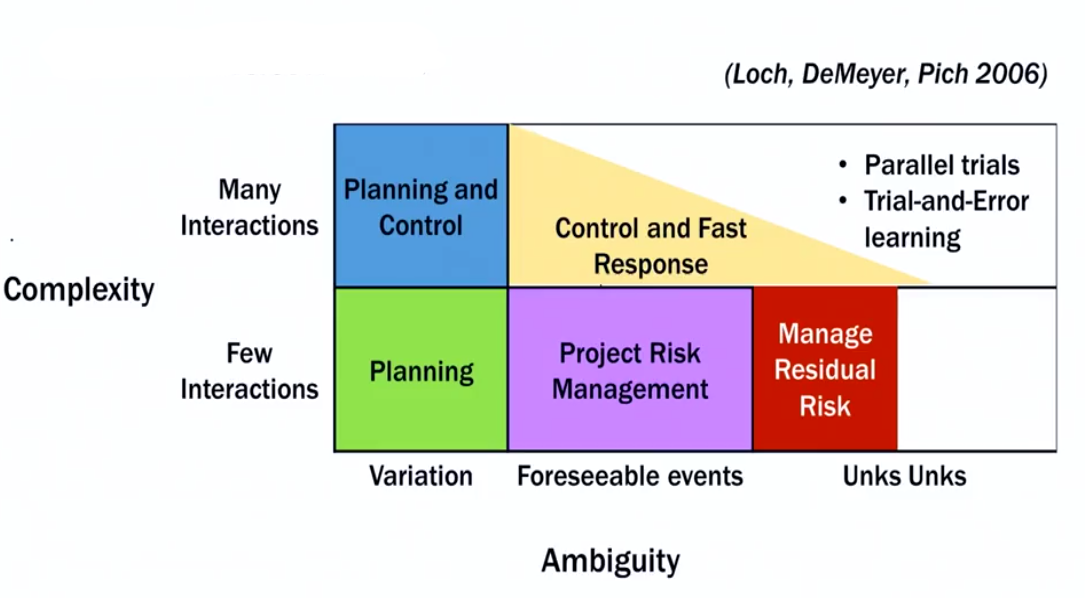
\includegraphics[width = 0.6\textwidth]{figs/fig5.png}
  \end{figure}
\end{frame}

\begin{frame}
 \frametitle{GRUPO DE PROCESSOS (“FASE”) – PLANEJAMENTO}
23 – Inter-relacionar as atividades e Definir Precedências- \\
Tipos de Inter-relacionamentos
  \begin{itemize}
   \item Término para término – TT (finish to finish – FF)
   \begin{itemize}
    \item A atividade sucessora somente termina com o final da atividade predecessora
    \item Essa relação faz com que as duas atividades finalizem sincronizadas
   \end{itemize}
  \end{itemize}
  \begin{figure}
   \centering
   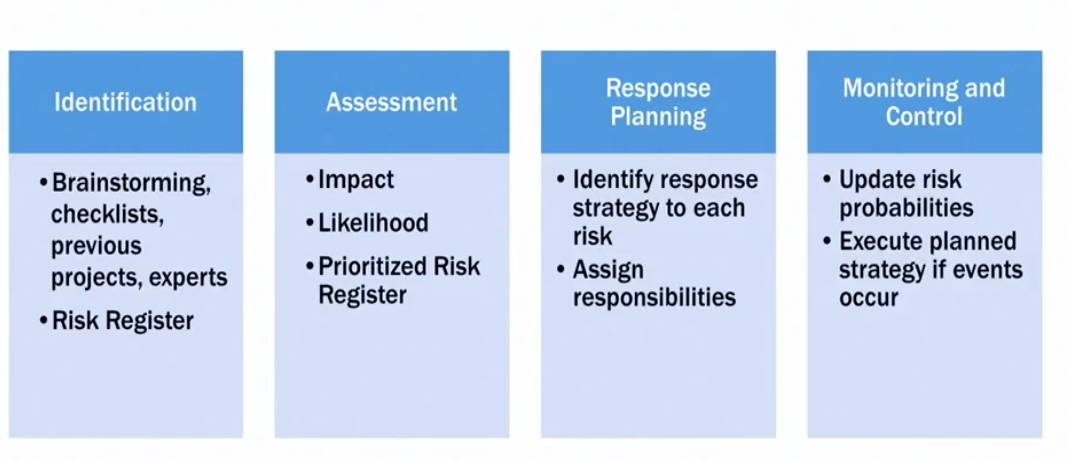
\includegraphics[width = 0.6\textwidth]{figs/fig6.png}
  \end{figure}
\end{frame}

\begin{frame}
 \frametitle{GRUPO DE PROCESSOS (“FASE”) – PLANEJAMENTO}
23 – Inter-relacionar as atividades e Definir Precedências-\\
Defasagem e Adiamento entre as atividades
  \begin{itemize}
   \item Diversas atividades necessitam de um intervalo de tempo após a realização de sua predecessora
   \item Não podem iniciar logo após a atividade anterior
  \end{itemize}
  \begin{figure}
   \centering
   
\includegraphics[width = 0.6\textwidth]{figs/fig7.png}
  \end{figure}
\end{frame}

\begin{frame}
 \frametitle{GRUPO DE PROCESSOS (“FASE”) – PLANEJAMENTO}
23 – Inter-relacionar as atividades e Definir Precedências- \\
Defasagem e Adiamento entre as atividades
  \begin{itemize}
   \item Tem o objetivo de adiantar o cronograma do projeto favorecendo a realização de atividades em paralelo
    \item O nome dessa técnica é \textbf{Paralelismo} ou \textbf{fast tracking}
      \end{itemize}
  \begin{figure}
   \centering
   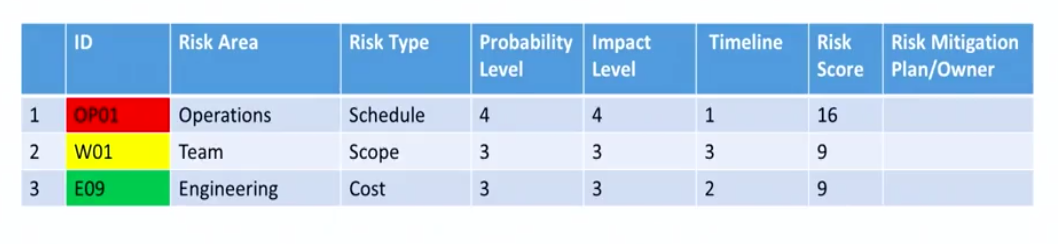
\includegraphics[width = 0.6\textwidth]{figs/fig9.png}
  \end{figure}
\end{frame}



\section{Calcular o Caminho Crítico}
\begin{frame}
 \frametitle{GRUPO DE PROCESSOS (“FASE”) – PLANEJAMENTO}
25 – Calcular o Caminho Crítico (CPM)
\begin{block}{}
 O Caminho crítico é definido como o caminho com a menor folga de tempo possível (usualmente zero) e determina a duração do projeto
\end{block}
  \begin{itemize}
   \item Atividades mais importantes
   \item Qualquer atraso no caminho crítico implica um atraso no término do projeto
   \item A duração do caminho crítico interfere diretamente na duração do projeto
  \end{itemize}
\end{frame}

\begin{frame}
 \frametitle{GRUPO DE PROCESSOS (“FASE”) – PLANEJAMENTO}
25 – Calcular o Caminho Crítico (CPM)
 \begin{itemize}
  \item Matriz de dependência com estimativa de tempo (ex Startup)
 \end{itemize}
  \begin{figure}
   \centering
   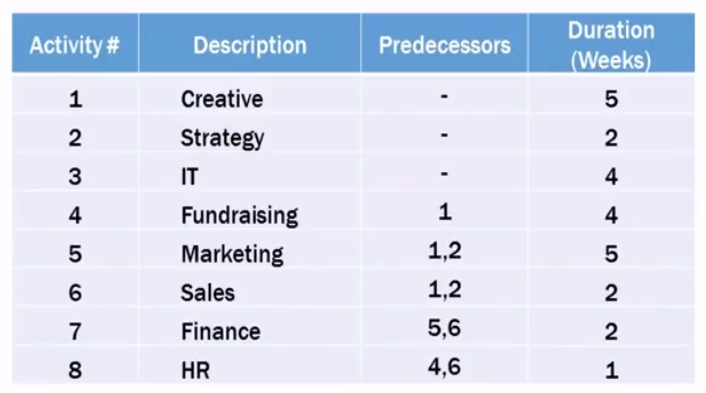
\includegraphics[width = 0.7\textwidth]{figs/fig24.png}
  \end{figure}
\end{frame}

\begin{frame}
 \frametitle{GRUPO DE PROCESSOS (“FASE”) – PLANEJAMENTO}
25 – Calcular o Caminho Crítico (CPM)
 \begin{itemize}
  \item Quanto tempo o projeto vai levar? (ex Startup)
 \end{itemize}
  \begin{figure}
   \centering
   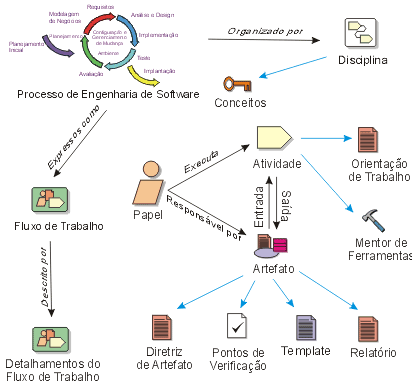
\includegraphics[width = 0.7\textwidth]{figs/fig25.png}
  \end{figure}
\end{frame}

\begin{frame}
 \frametitle{GRUPO DE PROCESSOS (“FASE”) – PLANEJAMENTO}
25 – Calcular o Caminho Crítico (CPM)
  \begin{itemize}
   \item Início mais cedo de uma atividade - IMC
   \begin{itemize}
    \item É a data de início mais \textbf{otimista} da atividade, sem que tenha ocorrido nenhum atraso
    \item Todas as atividades anteriores são realizadas adequadamente
    \item Todas as interdependências  com as predecessoras são respeitadas
   \end{itemize}
  \end{itemize}
\end{frame}

\begin{frame}
 \frametitle{GRUPO DE PROCESSOS (“FASE”) – PLANEJAMENTO}
25 – Calcular o Caminho Crítico (CPM)
 \begin{itemize}
  \item  Início mais cedo de uma atividade - IMC (ex Startup)
 \end{itemize}
  \begin{figure}
   \centering
   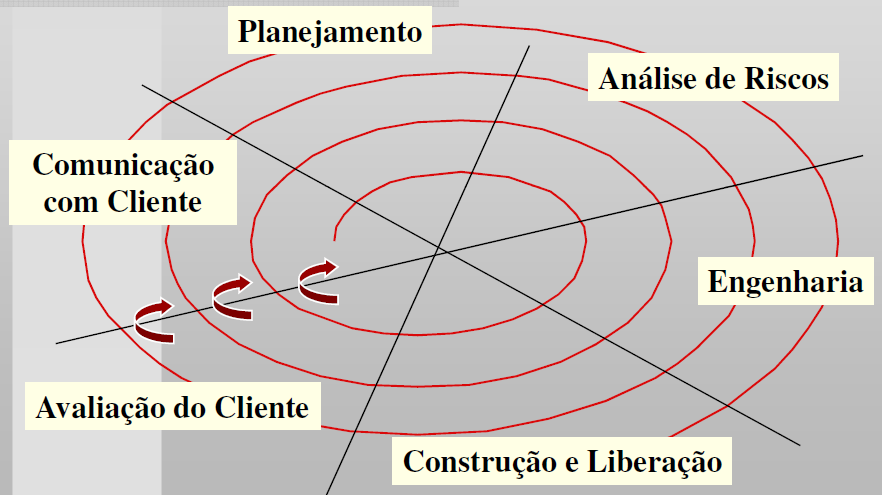
\includegraphics[width = 0.9\textwidth]{figs/fig26.png}
  \end{figure}
\end{frame}

\begin{frame}
 \frametitle{GRUPO DE PROCESSOS (“FASE”) – PLANEJAMENTO}
25 – Calcular o Caminho Crítico (CPM)
  \begin{itemize}
   \item Início mais tarde de uma atividade – IMT
   \begin{itemize}
    \item É a data de início mais \textbf{pessimista} da atividade, sem que, no entanto, o projeto seja prejudicado no todo
    \item É a última data em que se pode iniciar a atividade sem prejudicar o projeto
   \end{itemize}
  \end{itemize}
\end{frame}

\begin{frame}
 \frametitle{GRUPO DE PROCESSOS (“FASE”) – PLANEJAMENTO}
25 – Calcular o Caminho Crítico (CPM)
 \begin{itemize}
  \item  Início mais tarde de uma atividade – IMT(ex Startup)
 \end{itemize}
  \begin{figure}
   \centering
   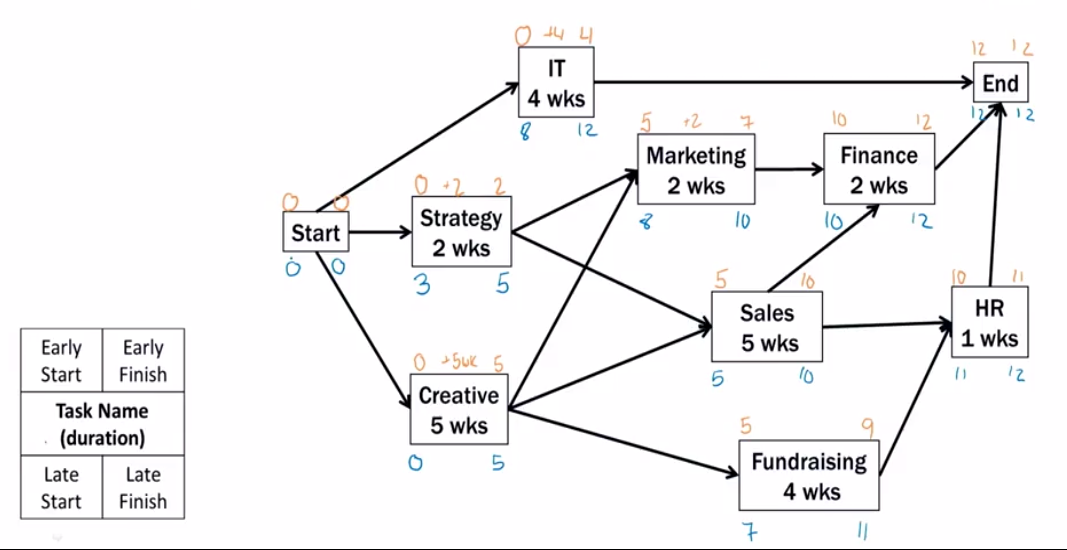
\includegraphics[width = 0.9\textwidth]{figs/fig27.png}
  \end{figure}
\end{frame}


\begin{frame}
 \frametitle{GRUPO DE PROCESSOS (“FASE”) – PLANEJAMENTO}
25 – Calcular o Caminho Crítico (CPM)
 \begin{itemize}
  \item  Caminho crítico (ex Startup)
 \end{itemize}
  \begin{figure}
   \centering
   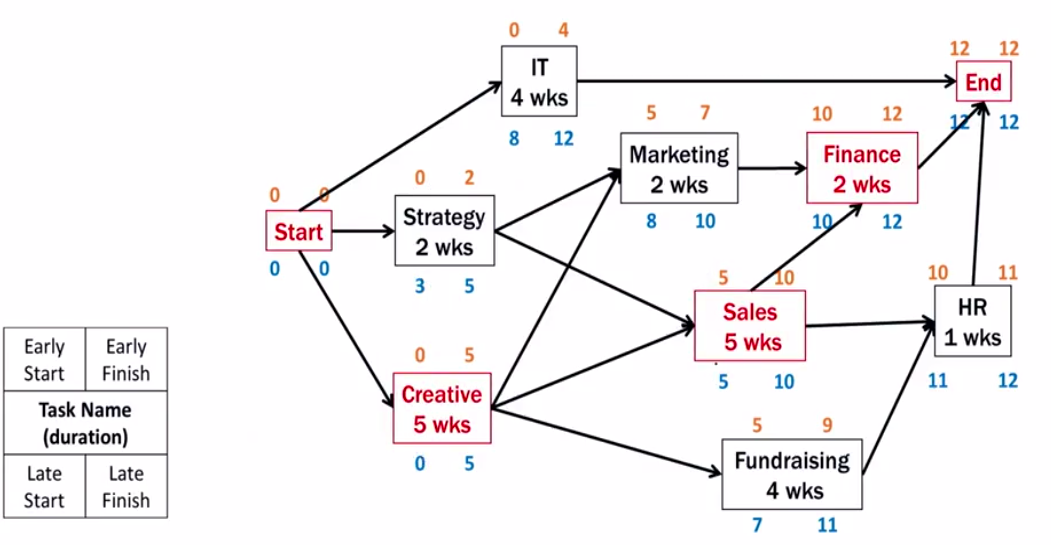
\includegraphics[width = 0.9\textwidth]{figs/fig28.png}
  \end{figure}
\end{frame}

\begin{frame}
 \frametitle{GRUPO DE PROCESSOS (“FASE”) – PLANEJAMENTO}
25 – Calcular o Caminho Crítico (CPM)
  \begin{itemize}
   \item Término mais cedo de uma atividade – TMC
   \begin{itemize}
    \item É a data de término mais \textbf{otimista} para atividade, não utilizando nenhuma folga
    \begin{equation}
     TMC = IMC + D
    \end{equation}
    onde TMC = término mais cedo \\
            IMC = início mais cedo  \\
            D = duração estimada
   \end{itemize}
  \end{itemize}
\end{frame}

\begin{frame}
 \frametitle{GRUPO DE PROCESSOS (“FASE”) – PLANEJAMENTO}
25 – Calcular o Caminho Crítico (CPM)
  \begin{itemize}
   \item Término mais tarde de uma atividade – TMT
   \begin{itemize}
    \item É a última data de término para atividade sem comprometer o término do projeto
    \begin{equation}
    TMT = IMT + D
    \end{equation}
    onde: TMT = término mais tarde \\
            IMT = início mais tarde\\
            D = duração estimada
   \end{itemize}
  \end{itemize}
\end{frame}

\begin{frame}
 \frametitle{GRUPO DE PROCESSOS (“FASE”) – PLANEJAMENTO}
25 – Calcular o Caminho Crítico (CPM)
  \begin{itemize}
   \item Folga Total – FT
   \begin{itemize}
    \item É a folga de tempo de uma atividade que não provoca nenhum atraso no \textbf{projeto}, podendo, no entanto, alterar as atividades \textbf{sucessoras}, desde que estas não sejam críticas
    \item Quando uma atividade utiliza toda FT, ela força, automaticamente, que todas as sucessoras diretamente ligadas a ela e tornem críticas
    \begin{equation}
   FT = TMT – IMT
    \end{equation}
    onde: FT = folga total \\
            TMT = término mais tarde \\
            IMT = início mais tarde
   \end{itemize}
  \end{itemize}
\end{frame}

\begin{frame}
 \frametitle{GRUPO DE PROCESSOS (“FASE”) – PLANEJAMENTO}
25 – Calcular o Caminho Crítico (CPM)
  \begin{itemize}
   \item FT para a atividade B é de 5 dias
   \item FT para a atividade C é de 3 dias
   \item FT para a atividade D é de 2 dias
   \item FT para a atividades A e E é zero
      \end{itemize}
  \begin{figure}
   \centering
   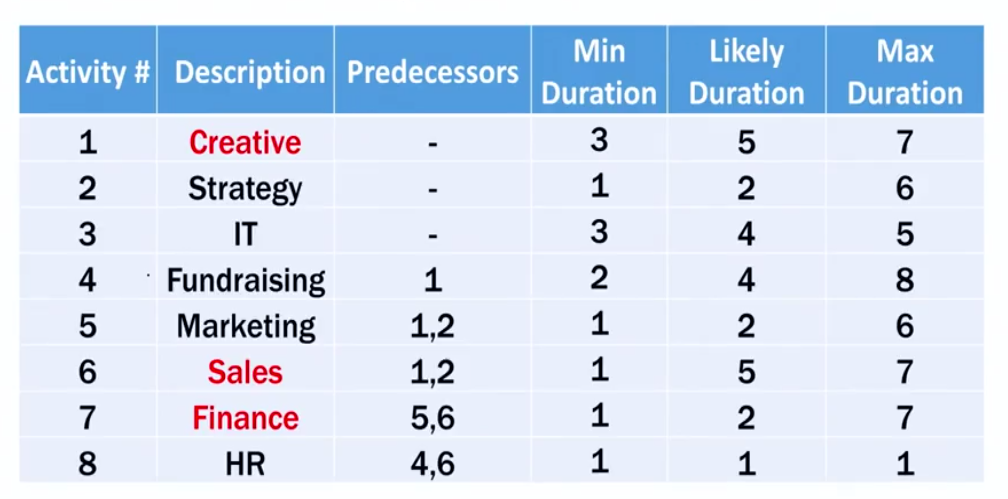
\includegraphics[width = 0.8\textwidth]{figs/fig10.png}
  \end{figure}
\end{frame}

\begin{frame}
 \frametitle{GRUPO DE PROCESSOS (“FASE”) – PLANEJAMENTO}
25 – Calcular o Caminho Crítico (CPM)
  \begin{itemize}
   \item Folga Livre ou Individual – FL
   \begin{itemize}
    \item É a folga de tempo de uma atividade de modo a não provocar nenhum atraso na atividade sucessora, independente dessa atividade ser ou não crítica
    \begin{equation}
      FL = IMC_j – TMC_i
    \end{equation}
onde: FL = folga livre \\
            TMCi = término mais cedo da predecessora \\
            IMCj = início mais cedo na sucessora \\
   \end{itemize}
  \end{itemize}
\end{frame}

\begin{frame}
 \frametitle{GRUPO DE PROCESSOS (“FASE”) – PLANEJAMENTO}
25 – Calcular o Caminho Crítico (CPM)
  \begin{itemize}
   \item FL para a atividade B é de 2 dias
   \item FL para a atividade C é de 1 dias
   \item FL para a atividade D é de 2 dias
      \end{itemize}
  \begin{figure}
   \centering
   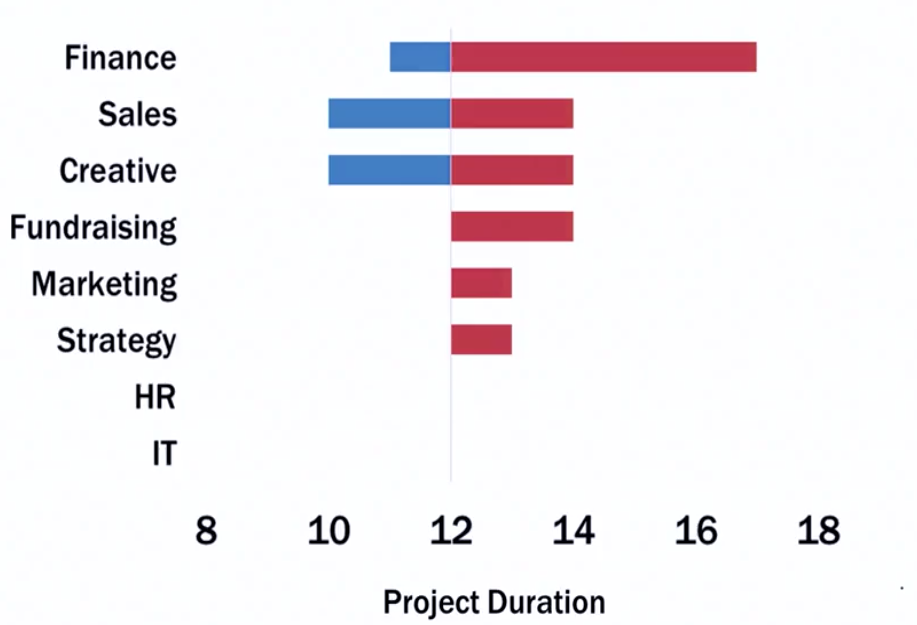
\includegraphics[width = 0.8\textwidth]{figs/fig11.png}
  \end{figure}
\end{frame}

\begin{frame}
 \frametitle{GRUPO DE PROCESSOS (“FASE”) – PLANEJAMENTO}
25 – Calcular o Caminho Crítico (CPM)
  \begin{itemize}
   \item Finalmente, destaca-se o caminho crítico, representado pelo caminho de atividades que apresenta menor folga ou folga zero
      \end{itemize}
  \begin{figure}
   \centering
   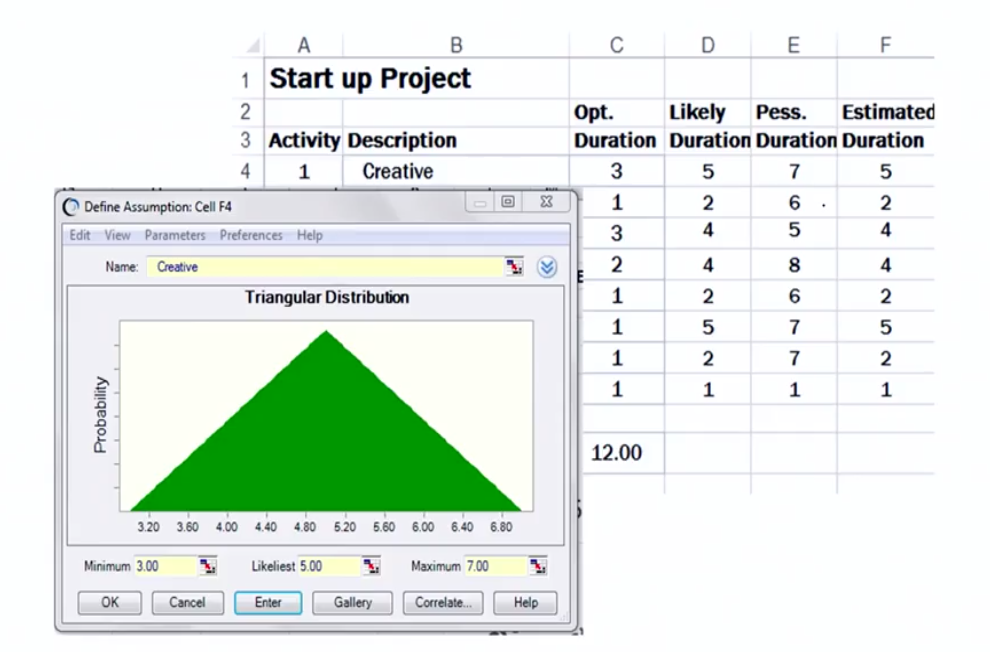
\includegraphics[width = 0.8\textwidth]{figs/fig12.png}
  \end{figure}
\end{frame}


\begin{frame}
 \frametitle{GRUPO DE PROCESSOS (“FASE”) – PLANEJAMENTO}
Checklist
  \begin{itemize}
   \item EAP-WBS
    \begin{enumerate}
     \item Disponível? Completo?
     \item Comunicado? Alinhado com principais stakeholders?
    \end{enumerate}
    \item Diagrama network
    \begin{enumerate}
     \item Um nó de início e um nó de fim?
     \item Todas as atividades tem predecessor e/ou sucessor?
    \end{enumerate}
    \item Milestones
    \begin{enumerate}
     \item Um milestone de início e outro no final do projeto?
     \item Milestones intermediários? Cada um com seu caminho crítico?
    \end{enumerate}

   \end{itemize}
\end{frame}

\section{Exercicio}
\begin{frame}
 \frametitle{EXERCÍCIO}
 \begin{itemize}
  \item Identifique quais são as atividades que ainda precisam ser refinadas ou realizadas no projeto da disciplina, a partir do fluxograma da “fase”de Planejamento
 \end{itemize}

\end{frame}


\end{document}
